\documentclass[../verslag.tex]{subfiles}
\graphicspath{{\subfix{../images/}}}
\begin{document}

Het model is gerepresenteerd als een Kripke-structuur. Hiervoor is UPPAAL gebruikt. UPPAAL is een programma dat is gemaakt om modellen te maken en te valideren.\\
Het meest overzichtelijk is om het model van de sluis op te delen in losse onderdelen. Deze onderdelen kunnen dan gecombineerd worden tot een complete sluis. De onderdelen van een sluis zijn de schutkolk, sluiscontroller, sluisdeuren en stoplichten.


\subsection{Onderdelen} 

\subsubsection{Sluiscontroller}
De sluiscontroller heeft 6 standen: GeschutL, DeurLOpen, DeurLDicht, GeschutR, DeurROpen en DeurRDicht.
Deze standen worden ook op deze volgorde geactiveerd om een cyclus van de sluis uit te voeren. Deze cyclus blijft zich herhalen.
\begin{figure}[H]
    \centering
    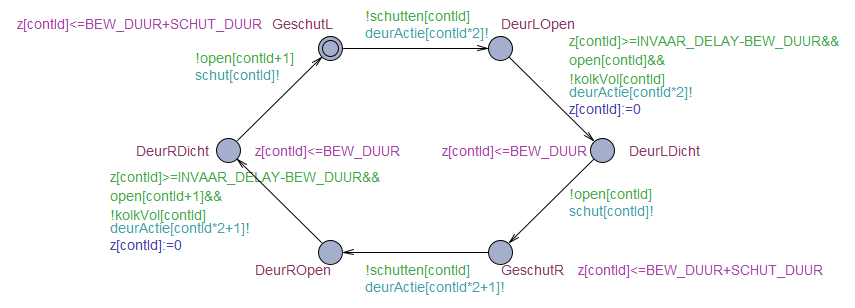
\includegraphics[width=1\textwidth]{model_sluiscontroller.png}
    \caption{Model van de sluiscontroller}
\end{figure}
De sluis start met beide deuren dicht en het water geschut naar het linker waterniveau. Dit is stand 'GeschutL'. Als de schutkolk niet aan het schutten is kan de linker deur opengedaan worden. Dit is stand 'DeurLOpen'. Vervolgens krijgen de boten tijd om de sluis uit en in te varen, en gaat de deur weer dicht na de invaar delay. Dit is stand 'DeurLDicht'. De deuren zijn gesloten na de bewegingsduur, de sluis begint dan te schutten naar het rechter waterniveau. Dit is stand 'GeschutR'. Als de sluiskolk klaar is met schutten kunnen de rechter deuren geopend worden. Dit is stand 'DeurROpen'. Het proces van links naar rechts werkt hetzelfde als van rechts naar links.

\subsubsection{Schutkolk}
Een schutkolk heeft 3 standen: LinkerNiveau, Schuttende en RechterNiveau.\\
Als het water in de schutkolk op het linker of het rechter niveau is kunnen boten uit en in de schutkolk varen. Het uit- en invaren van boten kan gedaan worden met transities op de standen van het linker en het rechter niveau. Als de schutkolk schuttende is, kunnen er dus geen boten in- of uitvaren.\\
Het aantal boten dat in de sluis past is afhankelijk van de CEMT-klasse. Deze klasse is in te stellen in de variabelen van de schutkolk.
\begin{figure}[H]
    \centering
    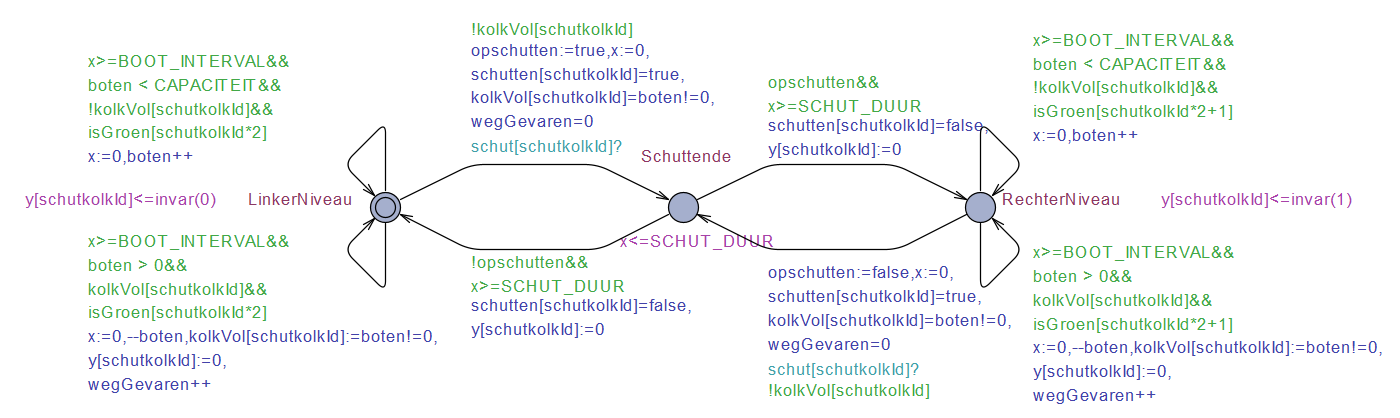
\includegraphics[width=1\textwidth]{model_schutkolk.png}
    \caption{Model van de schutkolk}
\end{figure}
Vanaf het linker niveau kunnen boten in de schutkolk varen als het linker stoplicht op groen is en als er plek is in de sluiskolk. (De sluisdeuren worden aangestuurd door de sluiscontroller.) Als de sluiscontroller aangeeft dat de schutkolk moet schutten gaat de schutkolk over in schuttende stand. Na de schut duur is het water op het rechter niveau. Als het rechter stoplicht op groen staat betekent het dat de sluisdeur open staat en dat de boten kunnen vertrekken. De boten moeten eerst vertrekken voordat er nieuwe boten in de schut kolk kunnen.

\subsubsection{Sluisdeur}
In het model van de sluis zijn altijd twee sluisdeuren aanwezig.
Een sluisdeur heeft 3 standen: Dicht, Bewegende en Open.
\begin{figure}[H]
    \centering
    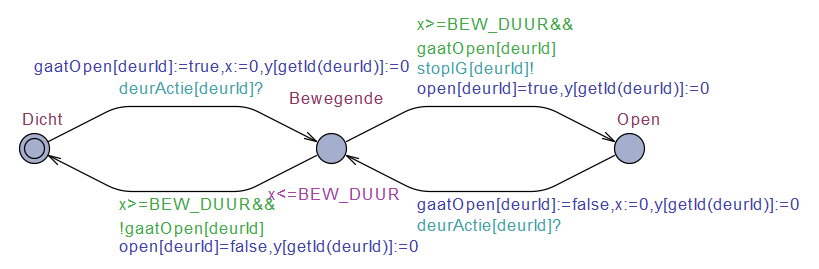
\includegraphics[width=1\textwidth]{model_sluisdeur.png}
    \caption{Model van de sluisdeur}
\end{figure}
Als de sluiscontroller het signaal geeft om de sluisdeur te openen gaat de deur bewegen. Na de bewegingsduur staat de deur helemaal open. Als de sluiscontroller het signaal geef om de sluisdeur te sluiten gaat de deur weer dicht.

\subsubsection{Stoplicht}
In het model van de sluis zijn altijd twee stoplichten aanwezig, een stoplicht per sluisdeur.
Een stoplicht heeft 2 standen: Rood en Groen.
\begin{figure}[H]
    \centering
    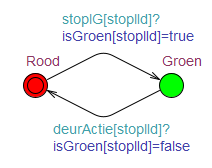
\includegraphics{model_stoplicht.png}
    \caption{Model van het stoplicht}
\end{figure}
Het stoplicht gaat op groen als de bijbehorende sluisdeur helemaal open is. Het stoplicht gaat weer op rood als de sluiscontroller de sluisdeur in beweging zet.


\subsection{Totaal model}
Het model bestaat uit vier verschillende onderdelen: sluisdeur, stoplicht, schutkolk en sluiscontroller. Deze werken samen door transities te synchroniseren. Het stoplicht gaat bijvoorbeeld op groen als de bijbehorende sluisdeur opengaat.\\
De transities in het model zijn tijdsgebonden. De sluis moet namelijk werken op een tijdschema. Ook kost het tijd om acties uit te voeren zoals de sluisdeuren openen of de sluis schutten. Globaal zijn variabelen aangemaakt om de duur van acties in te stellen. Zoals de cyclusduur, sluisdeur bewegingsduur, schutduur en de invaarduur.\\
Het model voor de sluis is modulair en makkelijk aan te passen. Het aantal boten dat in de sluis wordt toegelaten wordt bepaald door de CEMT-klasse en kan aangepast worden in de variabelen van de schutkolk. Het is ook mogelijk om meerdere sluizen te maken door dit in de globale declaraties aan te passen.


\end{document}
